{$\vx = \bmx{c}3\\1\emx$, $\vy = \bmx{c} 1\\-2\emx$}
{$\vx+\vy = \bmx{c}4\\-1\emx$, $\vx-\vy = \bmx{c} 2\\3\emx$

Sketches will vary depending on choice of origin of each vector.

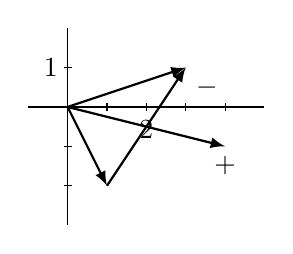
\begin{tikzpicture}[>=latex,scale=.5]
% Draw grid
\draw (-1,0)--(5,0);
\draw (0,-3)--(0,2);
\foreach \x in {1,...,4}
 {\draw (\x,-.1)--(\x,.1);
 }
\foreach \x in {-2,...,1}
 {\draw (-.1,\x)--(.1,\x);
 };
\node[below] at (2,-0.1) {2};
\node[left] at (0,1) {1};
%Draw arrows
\draw [->,thick] (0,0)--(3,1) node [above] {\vx};
\draw [->,thick] (0,0) -- (1,-2) node [below ] {\vy};
\draw [->,thick] (0,0) -- (4,-1) node [below] {$\vx+\vy$};
\draw [->,thick] (1,-2) -- (3,1) node [below right] {$\vx-\vy$};
\end{tikzpicture}
}